\documentclass[12pt]{article}
\usepackage[margin = 0.9in, top=0.8in]{geometry}
\usepackage{graphicx}
\usepackage{textgreek}
\usepackage{amsmath}
\usepackage{amsfonts}
\usepackage{mathtools}
\usepackage{amssymb}
\usepackage{float}
\usepackage{subcaption}
%\usepackage{algorithm}
%\usepackage{algorithmic}
%\usepackage[noend]{algpseudocode}
\usepackage[english]{babel}
\newtheorem{theorem}{Theorem}
\usepackage[ruled, lined, linesnumbered, commentsnumbered, longend]{algorithm2e}
\usepackage{hyperref}
\usepackage{grffile}
\graphicspath{{./2/images},{./2/data}, {./}}
\usepackage{hyperref}
\usepackage{grffile}
\graphicspath{{./2/images},{./}}
\title{CS 754 - Advanced Image Processing\\Assignment 4 - Report}
\author{Shaan ul Haque - 180070053\\Mantri Krishna Sri Ipsit - 180070032}
\newcommand{\norm}[1]{\left\lVert #1 \right\rVert}
\newcommand{\R}{\mathbb{R}}
\SetKwInOut{KwA}{Assumption}
\SetKwInOut{KwIn}{Input}
\SetKwInOut{KwOut}{Output}
\SetKwInOut{KwInit}{Initialization}
\SetKwInOut{KwIter}{Iteration}
\SetKwInOut{KwRep}{repeat}
\SetKwInOut{KwDef}{Define}
\begin{document}
	
	\maketitle
	
\section*{Question 1}
\subsection*{1.a and 1.b}
We used ISTA to estimate the sparse vector. The final function is sum of cosines, impulses and noise. Thus, the final signal is not sparse in either DCT basis or the temporal basis. In order to overcome this problem, we create an over-complete the dictionary which is concatenation of 256×256 DCT matrix and 256×256 identity matrix column wise. We varied the sparsity level of the signal, in their respective sparse domain, and then for each sparsity level varied the standard deviation of the noise. We calculated maximum Eigenvalue for the dictionary to be used in ISTA algorithm while the hyper-parameter $\lambda$ was chosen to be 1 as we observed least overall RMSE in the reconstructed signal. Plot for the RMSE error for both the signal f1 and f2 is given below.  
\begin{figure}[H]
	\centering
	\begin{subfigure}[b]{0.47\textwidth}
		\centering
		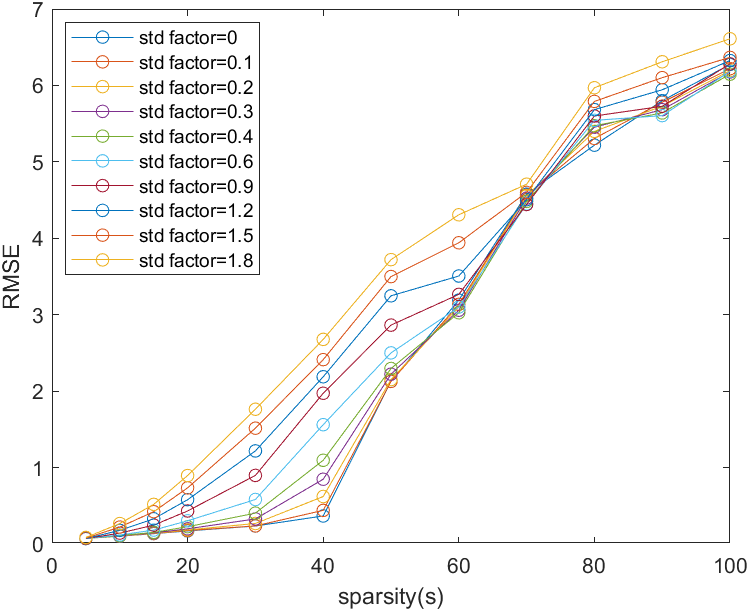
\includegraphics[width=\textwidth]{rmse_f1.png}
		\caption{$RMSE \ for \ f1$}
		\label{}
	\end{subfigure}
	\hfill
	\begin{subfigure}[b]{0.47\textwidth}
		\centering
		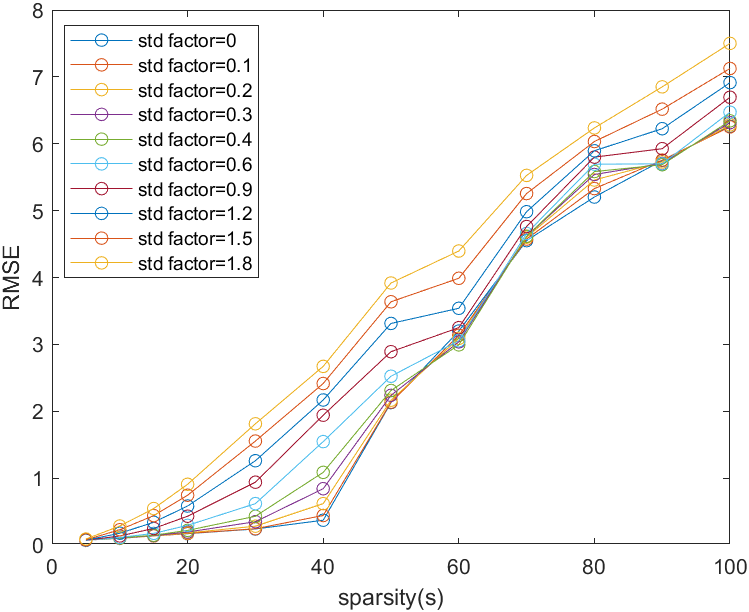
\includegraphics[width=\textwidth]{rmse_f2.png}
		\caption{$RMSE \ for \ f2$}
		\label{}
	\end{subfigure}
	\caption{RMSE}
	\label{fig:1}
\end{figure}
We observe that for same sparsity, increasing noise increases the RMSE error while increasing the sparsity level increases the noise as expected from the CS theorems. For large sparsity level(small S) typically in the range of 40 we observe that increasing noise has almost negligible effect on RMSE perhaps suggesting the small dependence of RMSE on noise variance (due to small S).
\subsection*{1.c}
We took sparsity level (s) = 20 and noise standard deviation factor = 0.5. We varied k from 0.1 to 10 in small steps initially and then larger steps subsequently. The figure shown below summarizes our result.
\begin{figure}[H]
	% will center the figure.
	\centering
	% include graphics (can include eps, jpg, pdf ...)
	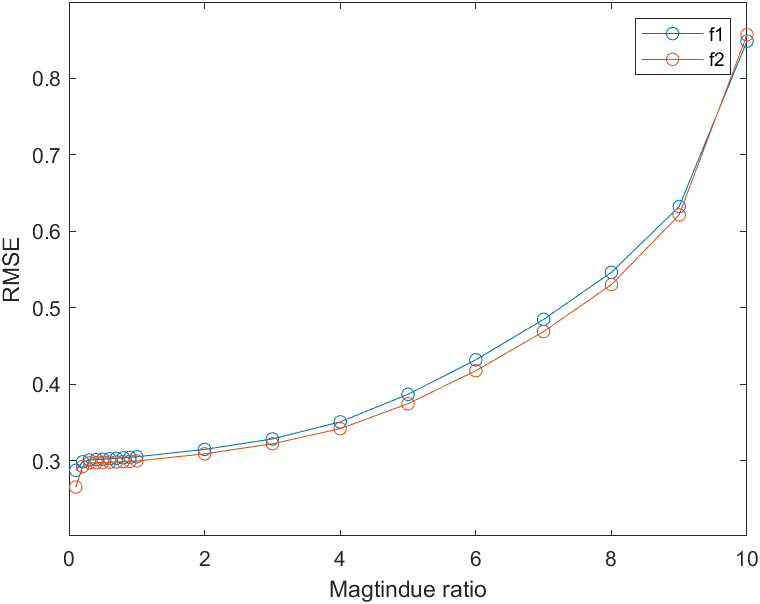
\includegraphics[scale=0.75]{rmse_mag.png}  % change scale factor to re-size the image.
	% give a caption.
	\caption{RMSE vs k}
	% a label to refer to the figure
	\label{fig:2}
\end{figure}
We observe that as we increase K the RMSE increases which is as we should expect since noise standard deviation = 0.5(mean(f1)+mean(f2)), thus as magnitude of f2 is increased noise variance increases as well leading to larger RMSE. The hyper-parameter $\lambda$ was chosen to be 1.75 as we observed least overall RMSE for this value.
	\section*{Question 2}
	The algorithm other than OMP and MP presented is called as \textbf{Look Ahead Orthogonal Matching Pursuit}. The standard OMP serially adds one component to the support-set that will irreversibly remain in the final estimate, in each iteration. The current choice of the component chosen is independent of the final result. This shortcoming can be overcome using a \textit{look ahead} strategy. In this method, an element is chosen by evaluating its effect on the final performance, in the sense of minimizing the fitting residual at the end of all future iterations. In the current iteration, several potential elements are chosen by the matched filter MF. Each of the potential elements are tested independently, and then one element among them is selected and inducted to the support-set. Among the potential elements, the element that will be selected provides the minimum fitting residual after executing all the future iterations (look ahead strategy). This method is referred to as LAOMP. To develop the LAOMP algorithm, the following algorithm is helpful:
	
	Some notations that were followed:
\begin{eqnarray*}
\texttt{resid}(\boldsymbol{y}, \boldsymbol{A}_{\mathcal{T}}) &\triangleq& \boldsymbol{y} - \boldsymbol{y}_p, \quad \text{where} \quad \boldsymbol{y}_p = \boldsymbol{A}_\mathcal{T}\boldsymbol{A}_\mathcal{T}^\dagger\boldsymbol{y}\\
\texttt{supp}(\boldsymbol{x}, k) &\triangleq& \text{\{the set of indices corresponding to the $k$ largest components of $\boldsymbol{x}$\}}\\
\texttt{supp}(\boldsymbol{x}) &\triangleq& \text{\{the set of indices corresponding to all the non-zero components of $\boldsymbol{x}$\}}
\end{eqnarray*}
	\begin{algorithm}[ht]
		\caption{\texttt{look\_ahead\_resid}: Look Ahead Residual}
		\KwIn{$\boldsymbol{A}, \boldsymbol{y}, T$, previous support-set $\mathcal{T}_{\text{old}}$, new index $\tau$}
		\KwA{$i \not \in \mathcal{T}_{\text{old}}$, $\hat{\boldsymbol{x}} \in \mathbb{R}^N$}
		\KwInit{}
		$k = |\mathcal{T}_{\text{old}}| + 1$\;
		$\mathcal{T}_k \gets \mathcal{T}_{\text{old}} \cup \tau$\;
		$\mathbf{r}_k \gets \texttt{resid}(\mathbf{y}, \mathbf{A}_{\mathcal{T}_k})$\;
		\KwIter{}
		\Repeat{k=T}{
		$k  \gets k+1$\;
	$\tau_k \gets \texttt{supp}(\mathbf{A}^{\intercal} \mathbf{r}_{k-1}, 1)$\;
$\mathcal{T}_k \gets \mathcal{T}_{k-1} \cup \tau_k$\;
$\mathbf{r}_k \gets \texttt{resid}(\mathbf{y}, \mathbf{A}_{\mathcal{T}_k})$\;}
\KwOut{$\mathbf{r} \gets \mathbf{r}_k$}
\end{algorithm}

The above algorithm is the look ahead part of LAOMP. Given the sparsity
level $T$ , an intermediate support set $\mathcal{T}$ and a new choice of an atom index $\tau$, the
algorithm usually finds a $T$-element support set at the end and returns the final least squares (LS) residual.	
\newline
The LAOMP algorithm is based on OMP to construct the support set progressively. In LAOMP, for the choice of a new atom, we take into account its effect
on the final performance in the sense of minimizing the residual. We fix an integer
parameter $\lambda$ which is referred to as the look ahead parameter. For the kth iteration,
the $\lambda$ best choices of new atoms are found using MF (Step 3). Then, for each choice
of $\lambda$ atoms, we allow the algorithm to execute until it selects $T$ atoms (Steps 4 and
5. From the $\lambda$ atoms we choose the one that results in the minimum norm of fitting
residual (Step 9). The chosen atom is added to the intermediate support set $\mathcal{T}_{k-1}$
to form the new support set $\mathcal{T}_k$ of cardinality k. The rest of the algorithm remains
same as standard OMP. We note that the algorithm must stop when the number
of iterations exceeds $T$ . Like most GP algorithms, we assume that the a-priori knowledge of the sparsity level $T$ is available. Also note that, as the value of the
look ahead parameter $\lambda$ increases, better performance can be expected, but at the
expense of higher complexity. For $\lambda = 1$, LAOMP will provide the same result as
OMP.
\begin{algorithm}[ht]
	\caption{Look ahead orthogonal matching pursuit (LAOMP)}
	\KwIn{$\boldsymbol{A}, \boldsymbol{y}, T$, look ahead parameter $\lambda \leq T$}
	\KwDef{$\boldsymbol{n} = [n_1, n_2, \ldots, n_\lambda]^\intercal$ and $\mathcal{T}_\Lambda = [\mathcal{T}_\Lambda(1)], \mathcal{T}_\Lambda(2), \ldots, \mathcal{T}_\Lambda(L)]$}
	\KwInit{}
	$k \gets 0, l \gets 0$\;
	$\boldsymbol{r}_k \gets \boldsymbol{y}, \hat{\boldsymbol{x}}_k \gets \boldsymbol{0}, \mathcal{T}_k \gets \emptyset$\;
	\KwIter{}
	\Repeat{k = T}{
	$k \gets k + 1$\;
$\mathcal{T}_\Lambda \gets \texttt{supp}(\boldsymbol{A}^\intercal\boldsymbol{r}_{k-1}, \lambda)$\;
\For{$l = 1$ to $\lambda$}{$\boldsymbol{rr} \gets \texttt{look\_ahead\_resid}\big(\boldsymbol{y}, \boldsymbol{A}, T, \mathcal{T}_{k-1}, \mathcal{T}_{\Lambda}(l)\big)$\;
$n_l \gets \norm{\boldsymbol{rr}}_2$}
$l \gets \text{Smallest component in \textbf{n}}$\;
$\tau_k \gets \mathcal{T}_{\Lambda}(l)$\;
$\mathcal{T}_k \gets \mathcal{T}_{k-1} \cup \tau_k$\;
$\hat{\boldsymbol{x}} \in \mathbb{R}^N$ such that $\hat{\boldsymbol{x}}_{\mathcal{T}_k} = \boldsymbol{A}^\dagger_{\mathcal{T}_k} \boldsymbol{y}$ and $\hat{\boldsymbol{x}}_{\mathcal{T}^c_k} = \boldsymbol{0}$\;
$\boldsymbol{r}_k \gets \texttt{resid}(\boldsymbol{y}, \boldsymbol{A}_{\mathcal{T}_k})$}
\KwOut{$\hat{\boldsymbol{x}} \in \mathbb{R}^N$ such that $\hat{\boldsymbol{x}}_{\mathcal{T}_k} = \boldsymbol{A}^\dagger_{\mathcal{T}_k} \boldsymbol{y}$ and $\hat{\boldsymbol{x}}_{\mathcal{T}^c_k} = \boldsymbol{0}$}
\end{algorithm}
As this algorithm is based on OMP, the following theorem which presents the performance bounds is also valid for LAOMP. (There is not seperate theorem stating performance bounds was given for LAOMP)
\newpage
\begin{theorem}
	Suppose that $\boldsymbol{A}$ satisfies the restricted isometry property (RIP) of order $T+1$ with isometry constant $\delta_{T+1} < \frac{1}{3\sqrt{T}}$. Then, for any $\boldsymbol{x} \in \mathbb{R}^N$ with the number of non-zeros less than or equal to $s$, LAOMP (OMP) will recover $\boldsymbol{x}$ exactly from $\boldsymbol{y} = \boldsymbol{A} \boldsymbol{x}$ in $T$ iterations.
\end{theorem}

\begin{theorem}[Restricted Isometry Property]
A matrix $A$ is said to obey the restricted isometry property of order $N$ if for any $N$-sparse vector $x$ 
$$(1 - \delta_N) \norm{x}^2_2 \leq \norm{Ax}_2^2 \leq (1 + \delta_N) \norm{x}_2^2$$
where $0 \leq \delta_N \leq 1$ is the smallest positive number such that the above relation holds and it is called ``restricted isometry constant" or ``isometry constant".
\end{theorem}
\section*{Question 3}
We know that by dictionary representation we can compactly express a large number image into small number of dictionary atoms. For any image, each of it's pixel value is the linear combination of those pixels in dictionary atom (when these atoms are represented into images by reshaping the columns). Due to this linearity, any linear operation done on the dictionary atoms gets reflected as it is in the image as well and vice versa. This can be seen from the following equations. \\
Let an image, $\boldsymbol{I} \in \boldsymbol{S}$, be represented by a linear combination of $s$ elements of a dictionary, given by $\boldsymbol{D} = \{\boldsymbol{d_1}, \boldsymbol{d_2}... \boldsymbol{d_k}\}$, that is the dictionary has total k atoms.
\begin{equation*}
	\boldsymbol{I} = \sum_{j=1}^{s} a_j\boldsymbol{d_{m_j}}  
\end{equation*}
where $a_j$ are the weights and $m_j$ are the column indices. If the dictionary atoms(columns) are reshaped into matrix, for each pixel in image we can observe that:
\begin{equation*}
	I(x,y) = \sum_{j=1}^{s} a_jd_{m_j}(x,y) \ \ \forall (x,y) \in \boldsymbol{I}
\end{equation*}
Let us perform any linear operation on the pixels of the image, mathematically:
\begin{equation*}
	f(I(x_l,y_l)) = \sum_{i=1}^{n}b_iI(x_{li},y_{li}) \ \ \forall (x_l,y_l) \in \boldsymbol{I}
\end{equation*}
where $(x_{li}, y_{li})$ are the spatial locations that the linear transformation takes into account (l and i will be related according to the linear transformation, for example $I(x_{li}, y_{li})$ might be the 8-neighborhood pixels around $(x_l, y_l)$, etc). Replacing $I(x_i, y_i)$, we get:
\begin{equation*}
	f(I(x_l,y_l)) = \sum_{i=1}^{n}b_i\sum_{j=1}^{s} a_jd_{m_j}(x_{li},y_{li})
\end{equation*}
Interchanging the summation:
\begin{equation*}
	f(I(x_l,y_l)) = \sum_{j=1}^{s}a_j(\sum_{i=1}^{n}b_i d_{m_j}(x_{li},y_{li}))
\end{equation*}
The term inside the brackets is the same linear operation albeit on the dictionary atoms. Thus we have shown that:
\begin{equation*}
	f(\sum_{j=1}^{s} a_jd_{m_j}(x,y)) = f(I(x_l,y_l)) = \sum_{i=1}^{s}a_jf(d_{m_j}(x_l,y_l)) 
\end{equation*}
\subsection*{3.a}
Any derivative filter on an image is a linear function of the pixels. Thus, as shown above, for the images in $\boldsymbol{S_1}$ the dictionary can be easily constructed using the  same derivative filter on the atoms of the $\boldsymbol{D}$ as used for the images in $\boldsymbol{S}$. Thus the newly formed dictionary will be $\boldsymbol{D_1} = \{f(\boldsymbol{d_1}), f(\boldsymbol{d_2})... f(\boldsymbol{d_k})\}$, where k is the number of dictionary atoms and \textit{f} is the derivative filter.
\subsection*{3.b}
Again, rotation of any image is linear transformation on the image pixels. But here we need slight tweaking in the sense there are two known angles, $\alpha$ and $\beta$, in which the images are rotated. Thus to overcome this issue we will rotate all the atoms (represented as images) by $\alpha$ and $\beta$ separately and then concatenated both the dictionaries column wise. The intuition behind this is same as we had for Question 1 of this assignment. If $\boldsymbol{D_{\alpha}} = \{\boldsymbol{d_{1\alpha}}, \boldsymbol{d_{2\alpha}}... \boldsymbol{d_{k\alpha}}\}$ and $\boldsymbol{D_{\beta}} = \{\boldsymbol{d_{1\beta}}, \boldsymbol{d_{2\beta}}... \boldsymbol{d_{k\beta}}\}$ represent rotated version of the columns (when represented in image form) then the final dictionary would be $\boldsymbol{D_{2}} = [\boldsymbol{D_{\alpha}} | \boldsymbol{D_{\beta}}]$.
\subsection*{3.c}
The given transformation is not linear in nature.
\begin{equation*}
	I_{new}(x,y) = \alpha(I_{old}(x,y))^2+\beta I_{old}(x,y)+\gamma
\end{equation*}
But we observe some pattern in the transformation which manifests itself in the dictionary as follows. Let the some image $\boldsymbol{I}\in \boldsymbol{S}$ be represented as:
\begin{equation*}
	\boldsymbol{I} = \sum_{j=1}^{s} a_j\boldsymbol{d_{m_j}}  
\end{equation*}
where the symbols have their usual meaning as defined earlier. Writing in pixel form we get:
\begin{equation*}
	I(x,y) = \sum_{j=1}^{s} a_jd_{m_j}(x,y) \ \ \forall (x,y) \in \boldsymbol{I}
\end{equation*}
Applying the quadratic transformation, we get:
\begin{equation*}
	I_{new}(x,y) = \alpha(\sum_{j=1}^{s} a_jd_{m_j}(x,y))^2+\beta(\sum_{j=1}^{s} a_jd_{m_j}(x,y))+\gamma 
\end{equation*}
Opening the square term, we get:
\begin{equation*}
	I_{new}(x,y) = \alpha(\sum_{j=1}^{s} a_j^2d_{m_j}^2(x,y)+2\sum_{i\not= j}a_ia_jd_{m_i}(x,y)d_{m_j}(x,y))+\beta(\sum_{j=1}^{s} a_jd_{m_j}(x,y))+\gamma 
\end{equation*}
Observing the above term, it is clear that the new dictionary must be concatenation of various functions of the dictionary columns. The new dictionary must have each column squared(element wise), pairwise product(element wise) of each column and a constant ones column(scaling will not matter as it will get absorbed in the coefficient). Thus new dictionary would be concatenation of:
\begin{equation*}
	\boldsymbol{D_{sq}} = \{\boldsymbol{d_1}^2, \boldsymbol{d_2}^2... \boldsymbol{d_k}^2\}
\end{equation*}
where $\boldsymbol{x}^2$ means element wise square of the vector. 
\begin{equation*}
	\boldsymbol{D_{pr}} = \{...\boldsymbol{d_i}\cdot\boldsymbol{d_j}...\} \ \ \forall i\not=j \ \ i,j\in \{1, 2, ... s\}
\end{equation*}
where $\boldsymbol{x\cdot y}$ means element wise product of the vectors.
\begin{equation*}
	\boldsymbol{D_c} = ones(\# \ of \ columns(D), 1)
\end{equation*}
Thus, $\boldsymbol{D_3} = [\boldsymbol{D_{sq}}| \boldsymbol{D_{pr}}| \boldsymbol{D}| \boldsymbol{D_c}]$

\subsection*{3.d}
Blur kernels are linear transformation on images only, such as the Gaussian blur filter. Thus as done for derivative filter, we can apply this known blur kernel to all the atoms of the dictionary(represented as images) to get the required dictionary. If \textit{f} is the known blur kernel, then the final dictionary $\boldsymbol{D_4} = \{f(\boldsymbol{d_1}), f(\boldsymbol{d_2})... f(\boldsymbol{d_k})\}$.
\subsection*{3.e}
Let the set of blur kernel $\boldsymbol{B} = \{\boldsymbol{b_1}, \boldsymbol{b_2}... \boldsymbol{b_p}\}$. Now let us pick any image $\boldsymbol{I_{blur}}$ from set $\boldsymbol{S_5}$ which is a blurred image of $\boldsymbol{I}$ from $\boldsymbol{S}$.
\begin{equation*}
	\boldsymbol{I_{blur}} = \sum_{i=1}^{n}c_i\boldsymbol{b_i(I)}
\end{equation*}
where $c_i$ is the weights for the blur kernel for the image. From part d, we know that blur kernel gets applied as it is to the atoms of the dictionary as well. Thus, all the new images in the set $\boldsymbol{S_5}$ are essentially linear combination of various blurred atoms from the dictionary with appropriate weights. The new dictionary will be concatenation of various blurred dictionary atoms, $\boldsymbol{D_5}$ = $[\boldsymbol{b_1(D)}| \boldsymbol{b_2(D)}|... \boldsymbol{b_p(D)}]$, where $\boldsymbol{b_i(D)} = \{\boldsymbol{b_i(d_1)}, \boldsymbol{b_i(d_2)}... \boldsymbol{b_i(d_k)}\}$, i.e., the blur kernel applied to all the atoms of the dictionary.
\section*{Question 4}
\subsection*{4.1}
$$J(\boldsymbol{A_r}) = \norm{\boldsymbol{A} - \boldsymbol{A_r}}_F^2$$
Solving this optimization problem is nothing but finding the best r-rank approximation of the matrix $\boldsymbol{A}$.  As we have seen in the lecture, this is done by using the top r-largest singular values and reconstructing $\boldsymbol{A_r}$. This is also known as \textbf{Eckart–Young–Mirsky theorem}. 
\begin{eqnarray*}
	\boldsymbol{A} &=& \boldsymbol{U} \boldsymbol{S} \boldsymbol{V}^\intercal \\
	\implies \boldsymbol{A_r} &=& \boldsymbol{U}(:,1:r) \boldsymbol{S}(1:r,1:r)\bigg(\boldsymbol{V}(:,1:r) \bigg)^\intercal
\end{eqnarray*}
\newline
This low rank matrix approximation can be used in \textbf{Texture Completion}. Generally the texture or any repeating pattern is captured by the low rank approximation. This optimization problem can be used to remove occlusions either from a photo or a video and do a robust repair, which is an application of \textbf{Robust PCA}.

\subsection*{4.2}
$$J(\boldsymbol{R}) = \norm{\boldsymbol{A} - \boldsymbol{RB}}_F^2$$
\vspace{1cm}
\begin{center}
	\textit{Please turn over}
\end{center}
\newpage
where $\boldsymbol{R}$ is an orthonormal matrix i.e, $\boldsymbol{R}\boldsymbol{R}^\intercal = \boldsymbol{R}^\intercal \boldsymbol{R} = \boldsymbol{I}$.
This optimization is solved as follows:
\begin{eqnarray*}
	\min \norm{\boldsymbol{A} - \boldsymbol{RB}}_F^2 &=& \min \mathrm{Tr}\bigg((\boldsymbol{A}-\boldsymbol{RB})^\intercal\, (\boldsymbol{A}-\boldsymbol{RB})\bigg)\\
	&=& \min \mathrm{Tr}\bigg((\boldsymbol{A}^\intercal-\boldsymbol{B}^\intercal\boldsymbol{R}^\intercal)\, (\boldsymbol{A}-\boldsymbol{RB})\bigg)\\
	&=& \min \mathrm{Tr}\bigg(\boldsymbol{A}^\intercal\boldsymbol{A}-2\boldsymbol{A}^\intercal\boldsymbol{RB} + \boldsymbol{B}^\intercal\boldsymbol{B}\bigg)\\
	&=& \max \mathrm{Tr}\bigg(\boldsymbol{A}^\intercal\boldsymbol{RB}\bigg)\\
	&=& \max \mathrm{Tr}\bigg(\boldsymbol{RB}\boldsymbol{A}^\intercal\bigg) \:\:\:\quad \text{since trace(PQ) = trace(QP)}\\
\text{using SVD on $\boldsymbol{BA}^\intercal$}\quad \boldsymbol{BA}^\intercal &=& \boldsymbol{UDV}^\intercal\\
&=& \max  \mathrm{Tr}\bigg(\boldsymbol{R}\boldsymbol{UDV}^\intercal\bigg)\\
&=& \max \mathrm{Tr}\bigg(\boldsymbol{V}^\intercal\boldsymbol{RUD}\bigg)\\
&=& \max \mathrm{Tr}\bigg(\boldsymbol{Z(R)}\boldsymbol{D}\bigg)\\
&=& \max \sum \limits_{i} z_{ii}d_{ii} \leq \sum \limits_{i} d_{ii} \quad (\because \boldsymbol{Z(R)}^\intercal \boldsymbol{Z(R)} = \boldsymbol{I})\\
\end{eqnarray*}
The maximum is achieved for $\boldsymbol{Z(R)} = \boldsymbol{I}$, i.e.,
$$\boldsymbol{R} = \boldsymbol{V} \boldsymbol{U}^\intercal$$

This algorithm is used in the \textbf{Tomography under unknown angles for 3D images}, where we try to estimate the rotation matrix $\boldsymbol{R}$. This problem is also known as \textbf{Orthogonal Procrustes} problem.
\section*{Question 5}
\subsection*{5.a}
The problem of hyperspectral unmixing is defined using the following constrained convex optimization problem:
$$\hat{\boldsymbol{s}}[n] = \arg \min \limits_{\boldsymbol{s}[n] \in \mathcal{S}} \norm{\boldsymbol{y}[n] - \boldsymbol{A} \boldsymbol{s}[n]}_2^2, \text{ such that } \sum \limits_{i=1}^N s_i[n] = 1, s_i[n] \geq 0, i=1, \ldots, N,\: n=1, \ldots ,L$$
where 
\begin{itemize}
	\item $\boldsymbol{y}[n] = [y_1[n], y_2[n], \ldots, y_M[n]]^\intercal \in \mathbb{R}^M$ is a vector of hyperspectral camera measurements where $y_m[n]$ denotes the camera's measurement at spectral band $m$ and pixel $n$. There are a total of $M$ spectral bands and $L$ pixels.
	\item $\boldsymbol{A} = [\boldsymbol{a}_1, \ldots, \boldsymbol{a}_N] \in \mathbb{R}^{M \times N}$ is called as the \textit{endmember matrix} and each $\boldsymbol{a_i}$ is called \textit{endmember signature vector} where $N$ is the total number of endmembers or the materials in the scene.
	\item $\boldsymbol{s}[n] = [s_1[n], \ldots,s_N[n]]^\intercal \in \mathbb{R}^N$ is called the \textit{abundance vector} at pixel $n$ where $s_i[n]$ describes the contribution of material $i$ at pixel $n$.
\end{itemize}
\subsection*{5.b}
We have the block model
$$\boldsymbol{Y} = \boldsymbol{A}\boldsymbol{S}, \boldsymbol{S} \in \mathbb{R}^{K \times L}, \boldsymbol{Y} \in  \mathbb{R}^{M \times L}$$
If $S$ denotes the set of indices of active materials in the measured data $\boldsymbol{Y}$, and if $\boldsymbol{A}_S$ denotes the matrix made from the columns of $\boldsymbol{A}$ indexed by $S$. If the set of true abundance maps $\{\boldsymbol{s}^i\}_{i \in S}$ are assumed to be linearly independent, then $\mathcal{R}(\boldsymbol{Y}) = \mathcal{R}(\boldsymbol{A}_S)$, where $\mathcal{R}$ denotes the range space of its argument. This gives us equation (40):
$$\norm{\boldsymbol{S}}_{\text{row -- 0}} < \text{spark}(\boldsymbol{A}) - 1$$
Here $\text{spark}(\boldsymbol{A})$ denotes the smallest number of linearly dependent columns of $\boldsymbol{A}$ and $\norm{\boldsymbol{S}}_{\text{row -- 0}}$ denotes the number of non-zero rows in $\boldsymbol{S}$. So, the problem requirements that we have are stated as follows:
\begin{itemize}
	\item $\boldsymbol{A} \geq 0$, $\boldsymbol{S} \geq 0$ (based on physical constraints) and $\boldsymbol{Y} = \boldsymbol{A}\boldsymbol{S}$. 
	\item As $\mathcal{R}(\boldsymbol{Y}) = \mathcal{R}(\boldsymbol{A}_S)$, we are trying to represent the columns of $\boldsymbol{Y}$ in the basis formed using columns of $\boldsymbol{A}$.
	\item As per the inequality mentioned above, we have $K < M$
\end{itemize}
All the above requirements are captured by performing NMF on $\boldsymbol{Y}$.

\subsection*{5.c}
Standard NMF may not guarantee solution uniqueness. This is a serious issue to the blind HU application, since it means that an NMF solution may not be necessarily be the true endmembers and abundances, even in the noiseless case. Hence, for the case of blind HU, NMF is modified to fit the problem better. The unified NMF-based blind HU problem can be formulated as follows:
$$\min \limits_{\boldsymbol{A} \geq 0, \boldsymbol{S} \in \mathcal{S}^L}\norm{\boldsymbol{Y} - \boldsymbol{A} \boldsymbol{S}}_F^2 + \lambda \cdot g(\boldsymbol{A}) + \mu \cdot h(\boldsymbol{S})$$
where $\mathcal{S}^L = \{\boldsymbol{S} | \boldsymbol{s}[n] \geq \boldsymbol{0}, \boldsymbol{1}^\intercal \boldsymbol{s}[n] = 1, 1 \leq n \leq L\}$, $g$ and $h$ are regularizers and $\lambda$ and $\mu$ are positive constants. The following two variations of blind HU are explained:
\begin{enumerate}
	\item \textbf{Iterated Constrained Endmember}(ICE):\newline
	Here, $h(\boldsymbol{S}) = 0$ and 
	$$g(\boldsymbol{A}) = \sum \limits_{i=1}^{N-1}\sum \limits_{j=i+1}^N \norm{\boldsymbol{a}_i - \boldsymbol{a}_j}_2^2$$
	which is the sum of differences between the vertices.
	\item \textbf{Sparsity Promoting Iterated Constrained Endmember}(SPICE):\newline
	$$g(\boldsymbol{A}) = \sum \limits_{i=1}^{N-1}\sum \limits_{j=i+1}^N \norm{\boldsymbol{a}_i - \boldsymbol{a}_j}_2^2$$
	$$h(\boldsymbol{S}) = \sum \limits_{i=1}^N \gamma_i \norm{\boldsymbol{s}^i}_1$$
	Here, we promote sparsity on the columns of $\boldsymbol{S}$
\end{enumerate}

\end{document}
